\documentclass[english]{article}
\usepackage{float}
\usepackage{graphicx}
\usepackage{needspace}
\usepackage{array}
\usepackage{varwidth}
\usepackage{caption}
\usepackage{babel}
\usepackage[paperwidth=20cm,paperheight=28cm,bottom=5em,top=5em]{geometry}
\usepackage[autostyle]{csquotes}
\usepackage{ragged2e}
\makeatother


\begin{document}
\pagestyle{empty}

%-------------------------------------------------
%	COVER PAGE
%-------------------------------------------------

\begin{center}
\textbf{\large A}{\LARGE{} }
\end{center}
%\vspace{2pt}44444
\begin{center}
\textbf{\LARGE B.TECH PROJECT PROPOSAL}{\LARGE{} }
\end{center}

\begin{center}
\textbf{\large on}
\end{center}

\begin{center}
\textbf{\Large Dudhganga Dairy Application for }\\
\vspace{8pt}
\textbf{\Large Milk Collector and Farmers}
\end{center}

\vspace{2pt}
\begin{center}
{\textbf{\large for} } 
\end{center}

\begin{center}
\textbf{\Large B.Tech. in Computer Science and Engineering}
\end{center}

\begin{center}
{ \textbf{\large Submitted to}} 
\end{center}
\vspace{2pt}
\begin{figure}[H]
\centering

\includegraphics[scale=0.8]{logo.jpeg}
\end{figure}

\vspace{2pt}
\begin{center}
\textbf{\Large Department of Computer Science and Engineering,}\\
\vspace{5pt}
\textbf{ \large Annasaheb Dange College of Engineering \& Technology,}\\
\vspace{8pt}
\textbf{ \large Ashta, Sangli.}
\end{center}{\Large \par}
\begin{center}
\textbf{(An Autonomous Institude Affiliated to Shivaji University Kolhapur)}
\end{center}

\vspace{2pt}

\begin{center}
{\textbf{by}} 
\end{center}

\begin{center}
\hspace{1cm}\textbf{\large   Mr. Nishant Krushnat Shingate(20132003)}
\end{center}
\begin{center}
\hspace{1.5cm}\textbf{\large Ms.Avanti Hanmant Pawar(20132005)}
\end{center}
\begin{center}
\hspace{0.5cm}\textbf{\large Mr.Abhishek Maruti Shinde(20132008)}
\end{center}
\begin{center}
\hspace{1.7cm}\textbf{\large Ms.Vaishnavi Dinkar Jadhav(19131042)}
\end{center}

\vspace{10pt}

\begin{center}
{ \textbf{Under the Guidance of}} 
\end{center}

\begin{center}
\textbf{\Large Prof. D. R. Kale}
\end{center}

\vspace{25pt}
\begin{center}
{\large \textbf{Academic Year}} 
\end{center}

\begin{center}
\textbf{\Large 2022-23}
\end{center}

\clearpage % Start a new page


%---------------------------------------------
%	ABSTRACT
%---------------------------------------------



%\begin{center}
%\textbf{\Large Abstract}
%\end{center}
\vspace{20pt}
\pagenumbering{roman}
\section*{Abstract}%
\addcontentsline{toc}{section}{\numberline{}Abstract}%
%\abstract{\addtocontents{toc}{\vspace{1em}} % Add a gap in the Contents, for aesthetics

Milk production is one of the most important factors for the rural economy of India.
Dairy Milk production is a highly and fast-growing sector in INDIA. India has traditionally been a low-cost milk producer due to inexpensive feeding and maintenance cost.There are many people involved in the milk production sector. The people are involved in this sector are the farmers, owner’s of collection centers and owner’s of dairy plants. 
Daily, farmers provide milk to milk collectors, but most of the collectors follow unfair regarding weight and fat. Because of malpractice in measures of milk, there is no transparency between farmers and milk collectors about the accuracy and precision in the accounting and billing.
\\\\
\textbf{Keywords:} Milk, Fat, Weight, Dudhganga, Automation, Dairy, Farmers.



\clearpage % Start a new page

\tableofcontents

\pagenumbering{arabic}

\clearpage

\section{Introduction} % creates a section
Most local milk collectors in the small towns and villages collect milk and write down the fat and quantity of milk on the paper and at the time of bill calculation bill collectors calculate the bill of each customer by using a regular math calculator. Milk collector not only keep record of collected milk but also manages records of milk buyers, farmers and also keep account of cattle food provided to farmers with their money transactions. This process consumes more time to do all this calculation, and this time can be saved if we automate this process.So we are going to develop one application which will handle all of the work of the milk collector which he/she does manually.\\

\section*{Advantages} % creates a section
\begin{itemize}
\item Time saving for farmer milk collectors.
\item Data of milk is correctly updated to farmers on a daily basis.
\item Payment is directly credited to farmers' bank accounts after the specific 
 period.
\item Data is securely stored on the database.
\item  Device independent application.
\item User friendly applications.
\end{itemize}

\section*{Disadvantages} % creates a section
\begin{itemize}
\item Without an internet connection the application will not save data on the
database .
\item Input data about milk must be manually entered by the milk collector.\\

So, for all the above following discussed advantages and disadvantages we are going to provide an efficient solution to all the following demerits and will work for the most convenient product.
\end{itemize}

\subsection{Background and Context}
The system is for visually challenged people, and keyboard operations are completely avoided. Composing mail would only be done on voice input. No typed input will be required. Users can directly record messages that need to be generated and can send them. This voice message will go in the form of an attachment. The receiver can hear the recording and get the message the user wanted to send. Users would not require users to attach the file. Recording options will be provided in the composing window itself. Once recorded, it will confirm whether the recording is perfect or not by letting the user hear it, and if the user confirms it, it will be automatically attached to the mail. 
\subsection{Purpose}
Manually calculation of milk bill of each customer will consume more time and writing all the information about milk collected on the paper which needs the papers. This all is more costly.There are high changes of loosing data written on the paper. So the purpose of the Dudhganga Dairy application is to save the time of milk collector and save the cost of papers.
\\\
\clearpage
\section{ Brief Literature Review} % creates a section
\textbf{(A)	Existing Systems} \\
There are many existing system available with some features. Following are the some systems:
\item \textbf{1. The Shubhdra Dairy Management Software}\\
The Shubhra Dairy Management Software is a software which is used for dairy management with following features.
\begin{itemize}
\item  User-friendly billing system.
\item  Add daily milk details
\item Customer Management.
\item Billing Management
\item Report generation.

\end{itemize}
\item \textbf{2. Meri Dairy is another one Milk Collection center software for dairy owners with following features:}

\begin{itemize}
\item With every entry, Dairy customer will receive a test message (SMS)
\item TVS mini printer Available to print a daily receipt.
\item Payment Register
\item Daily report
\item Data saved on the server will be secure in case you lost your laptop/mobile. \item Customer app to watch their own records on the app
\item  Milk Sale purchase record.
\item  Complete FAT/SNF or CLR management

\end{itemize}
\textbf{(B)	Articles from International peer reviewed journals} \\
This material serves as a guide and update for readers working in the Character Recognition area.\\
A.	Ronak Chudasam, Sagar Dobariya (2017) [1]  This paper addresses the problem of analyzing data collected by the dairy production with the aim of optimizing the supply chain management and maximizing profit in the manufacturing of milk and other dairy items. The amount of data from dairy records continuously increases due to the usage of modern systems in farm management, requiring a technique to show trends and insights in data for a rapid analysis\\
B.	Jamshed Memon; Maira Sami; Rizwan Ahmed Khan;Mueen Uddin (2020)[2] This paper explores and develops the design method of Dairy Cow Data Acquisition System based on PDA. According to the application of the system, it proves that this system not only saves manpower, improves work efficiency and overall benefits, and at the same time it solves the problem of its combining with management system, provides timely and effective information and technical support to the directors' decision-making, improves the capacity of reacting to emergencies, and offers enormous technical support for the standardization of Islamic feeding of livestock husbandry, the informationization of management process, the automatic data collection of milk yield as well as the traceability of Islamic animal products. So the paper is innovative and of practical use to some extent.
 

\\\\

\clearpage
\section{Problem Statement} % creates a section
To design and develop a cross platform application for the automation of daily and routine activities of milk collection centers and farmers and milk buyers.\\
\item \textbf{• IDEAL:}
There must be transparency in the daily and routine transactions between the farmers and milk collectors. The process of calculation should be automated to avoid the miscalculation in accounting.
\item \textbf{• REALITY: }
In the rural areas, local milk collector’s collects milk and write the quantity of milk and fat of milk on paper for each customer. After the 10 days, they spend time to calculate the bill of each customer by taking the price depending on weight and fat for the respective milk of the customer. This whole process of bill calculation take average 5 for 6 days. And they also manage the records of payment of milk buyer on the notebook.
\item \textbf{• CONSEQUENCES:}
The current process at milk collection centers may lead to mal- practice while taking the readings. The current process of bill calculation many times leads to wrong calculation. Due to all these issues, the farmers have no belief on the milk collection centers. Daily and routine transactions are not transparent to milk producers.
\item \textbf{• PROPOSAL: }
The Dudhganaga Dairy application will be a cross platform application for the automation of daily and routine activities of milk collection centers and milk buyers. The Dudhganga Dairy application will also connect the milk collection centers and the farmer.



%\end\item\textbf{}

\section{Objectives} % creates a section
\begin{itemize}
\item To Design and develop the Database system for efficient storage and retrieval of data.
\item To Design and develop a friendly multilingual user interface for reading of weights and
    measures of milk at the collection center.
\item To Design and develop a messaging system to provide required alerts to farmers, milk
     collectors and dairy plants.
\item To analyze the data, prepare the bills daily/monthly/quarterly/annual reports.
\item To design & and develop systems which handle multiple users.\end{itemize}

%\section{Scope} % creates a section
%Tell readers the amount of detail you plan to cover. State the limitations if any

\section{Proposed Work} % creates a section
\subsection{Methodology}
\begin{itemize}
\item To make this app, multi language, first we have to translate each sentence in respective language.
\item The App will be available to use in the following languages:
1. English.
2. Marathi.
\item For storing the data related to the milk of each customer and information of each customer, we will be using the Firestore database provided by Google for Android Apps.
\item In Firestore the Complex, hierarchical data is easier to organize at scale, using sub- collections within documents
\item Figure 1 shows the collection and document Structure of the Dudhganga Dairy Application
\end{itemize}
\begin{figure}[H]
\centering
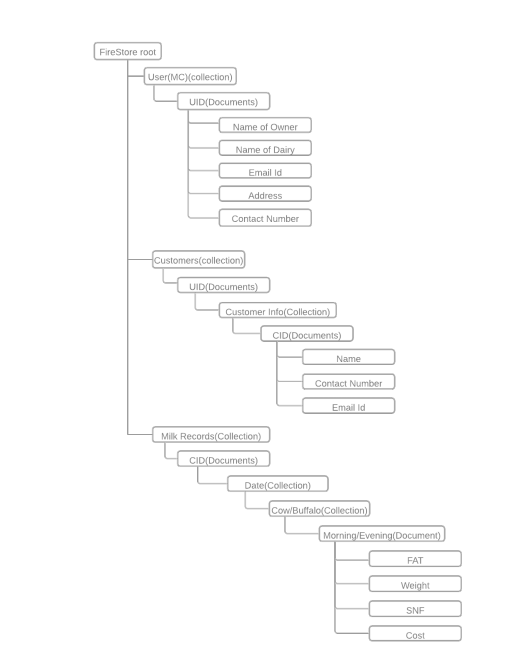
\includegraphics[scale=0.5]{database.png}
\caption{Firestore Database Structure for the Project}
\end{figure}
\begin{itemize}
\item To send the information about reading the milk and the bill of milk, we have designed another account separately for the farmer. By login to this app using the collection center name with unique key and password, they can see their records about the milk.
\item The inputs are taken two times in a day, at morning and evening, and stored on the database.
\item After the completion of 10 days. This software will automatically start the calculation of bills for each customer
\item	The values of prices of milk are predefined, So we will consider all that values while calculating total cost of milk.
\item The calculation will be done on the following things:\\
•	Cost of milk with respect to fat on each morning and evening,
cost of day = cost of morning milk + cost of evening milk\\
•	Then the cost of milk for 10 days will be calculated using the cost of each previous 10 days.\\
•	If the inputs are not given to the software, then it will consider the cost as 0 for that respective time and customer.\\
\end{itemize}
\begin{figure}[H]
\centering
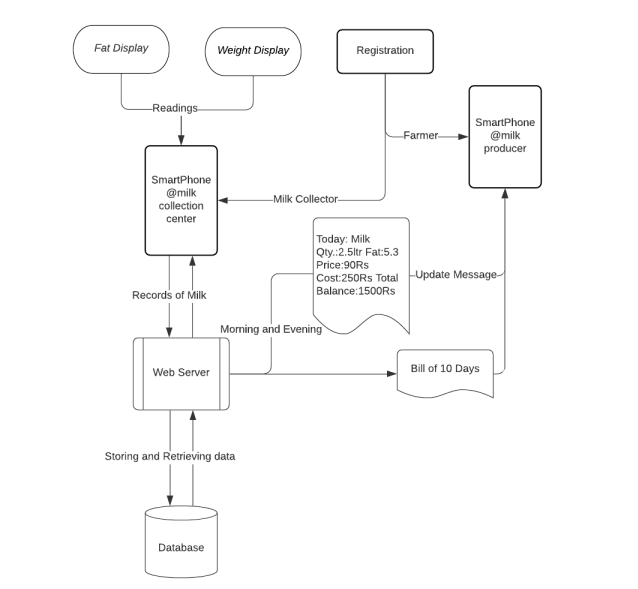
\includegraphics[scale=0.5]{databse 1.png}
\caption{Workflow diagram of Application }
\end{figure}




\subsection{Software and Hardware requirements and availability}
\hfill\break
\hspace{1cm}\normalsize\textbf{Software requirements}
\begin{itemize}
%\item \textbf{IDE:} Spyder
%\item \textbf{Coding language:} Python Version 3.8
%\item \textbf{Operating System:} Windows 10
%\item \textbf{Framework:} Django\\
\item 	Windows 10/Android/iOS/MacOS/Linux.
\item  Android Studio/Visual Studio, Flutter Framework, Firebase
\item	Dart Language.
\end{itemize}

\hspace{-0.5cm}\normalsize\textbf{Hardware requirements:}
\begin{itemize}
\item 8GB RAM(Minimum)
\item Memory 20GB
\item Core I5 processor
\\

\end{itemize}
\hspace{-0.5cm}\normalsize\textbf{Other requirements:}
\begin{itemize}
\item  Internet Connection Required
\end{itemize}
\\

%\section{Schedule} % creates a section
%In this section, provide the project plan in the stipulated period.
%\begin{itemize}
%\item Split entire work into subtasks such as literature survey, planning, development, installation, testing, writing reports or articles
%\item Precisely mention the timeline
%\item Prepare Gantt Chart - Type of bar chart that illustrates a project schedule -  - Use some tool for this
%\end{itemize}

%Figure 2 shows the project schedule to be used to implement the project.

%\begin{figure}[H]
%\centering
%\includegraphics[scale=0.8]{schedule.jpg}
%\caption{Project Schedule}
%\end{figure}

\section{Schdeule} % creates a section
\addcontentsline{toc}{section}{References}

\section*{References}
\vspace{20pt}

\begin{itemize}
\item[][1]	Ronak Chudasam, Sagar Dobariya (2017), “DAPS: Dairy analysis and prediction system using technical indicators”.

\item[][2]	Jamshed Memon; Maira Sami; Rizwan Ahmed Khan; Mueen Uddin (2020) “The dairy cattle data acquisition system based on PDA”

\end{itemize}

\vspace{20pt}

\section*{Group Members}
\vspace{20pt}

\centering
\begin{tabular}{ | c | c | c | c | c | c |}
     
\hline \bf{Sr.NO} &\textbf{Name of the Student} &\textbf{Contact No.} &\textbf{Email ID} 
&\textbf{Signature}  \\ 
     \hline   1 &Nishant Krushnat Shingate&8329060009&nishantks12@gmail.com &\\ 
     \hline   2 &Avanti Hanmant Pawar&7972824669&iamavantipawar@gmail.com&\\ 
     \hline   3 &Abhishek Maruti Shinde&9503648381&abhishekshinde9503@gmail.com &    \\
     \hline   4 &Vaishnavi Dinkar Jadhav &9763463876 &vaishanavijadhav1234@gmail.com & \\ 
    % \hline   & & & &\\
     \hline
    
      
\end{tabular}


\vspace{20pt}

\begin{FlushLeft}
Date: \today 
\\
\vspace{20pt}
Place: Ashta
\end{FlushLeft}
\normalsize\textbf{Prof.D. R. Kale} \hfill\normalsize\textbf{Prof.A. N. Jadhav} 


	\hspace{1cm}\normalsize\textbf{Guide}\hfill   \normalsize\hspace{3cm}\textbf{Project Coordinator}

\hfill\break
\begin{center}

	\normalsize\textbf{Prof.S. S. Sayyad }

	\normalsize\textbf{HOD, CSE}
\end{center}

\clearpage % Start a new page



\end{document}
